
\section{Headtracking}

Ziel des Headtrackings ist es, die Kopforientierung des Fahrers --~auch bei bewegtem Fahrzeug~--
%\todo{``fahrendem'' statt ``bewegendem''?}
% -> ich würde bei bewegt bleiben: es ist ja denkbar, dass das Auto nicht selber "fährt", aber trotzdem "bewegt" wird, beispielsweise auf einer Fähre oder so
sowohl relativ zum Fahrzeug als auch in Weltkoordinaten anzugeben. Unter Orientierung wird hier die Drehung entlang der X- (\emph{Roll}), Y- (\emph{Pitch}) und Z-Achse (\emph{Yaw}) verstanden:
\acs{RPY}.

Dazu wird die Inertialsensorik der \ac{AR}-Brille, bestehend aus zwei Gyroskopen, Beschleunigungssensor und Magnetometer, ausgewertet (Abs. \ref{headtracking_imu_subsec}).
Diese Daten werden mit einem geeigneten Filter-Algorithmus fusioniert (Abs.~\ref{headtracking_fusion_subsec}).
Die Kompensation der Eigenbewegung des Fahrzeugs wird in Abs. \ref{headtracking_marker_subsec} behandelt.

\subsection{Inertialsensoren}
\label{headtracking_imu_subsec}
Im folgenden Absatz werden die verschiedenen Sensoren vorgestellt. Dabei sei angemerkt, dass die gemessenen Daten in einem sogenannten \textit{Sensorkoordinatensystem $TF_{sensor}$} erfasst werden. Dieses ist um etwa $15^\circ$ in der Z-Achse rotiert zum \textit{Brillenkoordinatensystem $TF_{glasses}$}, welches seinen Ursprung in der Mitte des Brillenstegs hat. Dieses Koordinatensystem wurde so gewählt, dass es in etwa mit der Kameraposition der Brille übereinstimmt \footnote{Anbetracht der vorhandenen Messungenauigkeiten wurden die Translationen zwischen Sensor und Brillensteg sowie Kamera und Brillensteg vernachlässigt, da sie keinen eklatanten Einfluss auf die Orientierung der Brille bzw. des Kopfes haben.}. In Abb. \ref{fig:tf_baum_sensorik}

\todo[inline]{Ich bitte den Ersteller des TF-Baums sich dieser Grafik anzunehmen, der sieht sehr professionell aus, so was in abgespeckter Form brauchen wir hier auch, damit wir uns in den nachfolgenden Sections drauf beziehen können, bitte die Textreferenzen in \ref{headtracking_imu_subsec} dazu anpassen.}

\subsubsection{Gyroskop}
\label{headtracking_imu_gyro_subsubsec}

Das in der Brille enthaltene Gyroskop misst Winkelgeschwindigkeiten in
$\omega = [{Grad \over Sekunde}]$ bei Drehungen um die X-, Y- und Z-Achse. Durch
die Integration der Winkelgeschwindigkeiten über die Zeit kann die
Orientierung der Brille bestimmt werden.  

Die \ac{IMU} der Brille enthält zwei
Gyroskope, ein \emph{High Bandwidth} Gyroskop sowie ein
\emph{Low Bandwidth} Gyroskop. Die Gyroskope unterscheiden sich
hinsichtlich der Genauigkeit und des Wertebereiches. Das \ac{HBW}-Gyroskop
hat einen größeren Wertebereich, jedoch die geringere
Genauigkeit.

Die Rohdaten des Sensors enthalten einen konstanten Versatz, so dass bei
stationärer Brille eine Geschwindigkeit $\omega \neq 0$ gemessen wird.
Dieser Versatz wird \emph{Bias} bezeichnet, und muss in einem
stationären Kalibriervorgang ermittelt werden. Dazu werden die
Sensordaten über einen kurzen Zeitraum bei unbewegter Brille erfasst und
über die Zeit gemittelt. Der so ermittelte Wert wird von den
Sensor-Rohdaten subtrahiert. Abb. \ref{fig:gyro_bias} zeigt die Daten vor
und nach der Bias-Korrektur.

\begin{figure}[h]
   \centering
   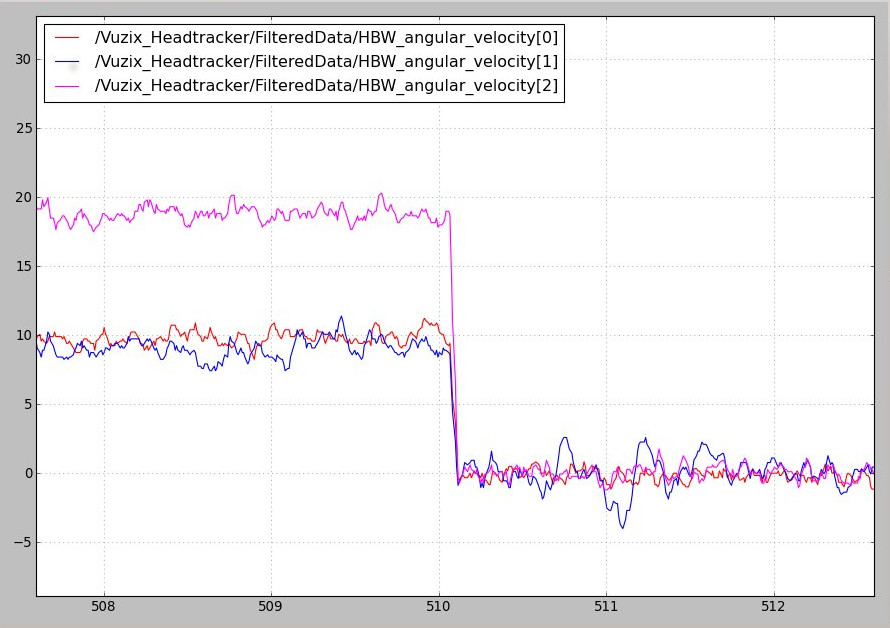
\includegraphics[width=0.45\textwidth]{stationary_calibration_before_after}
   \caption{Korrektur des Gyroskop-Bias}
   \label{fig:gyro_bias}
\end{figure}

Des Weiteren unterliegen die Sensordaten einem Rauschen. Daher wird als
nächster Schritt ein Tiefpassfilter verwendet, um dieses Rauschen zu
reduzieren. In unserem Fall hat sich ein Mittelwertfilter mit einer 
Fenstergröße von 5 als praktikabel erwiesen. Je höher die Fenstergröße gewählt wird,
desto stärker werden die Rohdaten geglättet, damit steigt jedoch auch
die Verzögerung der Daten. Abb. \ref{fig:lowpass-delay} zeigt den Effekt des Tiefpassfilters.

\begin{figure}[h]
   \centering
   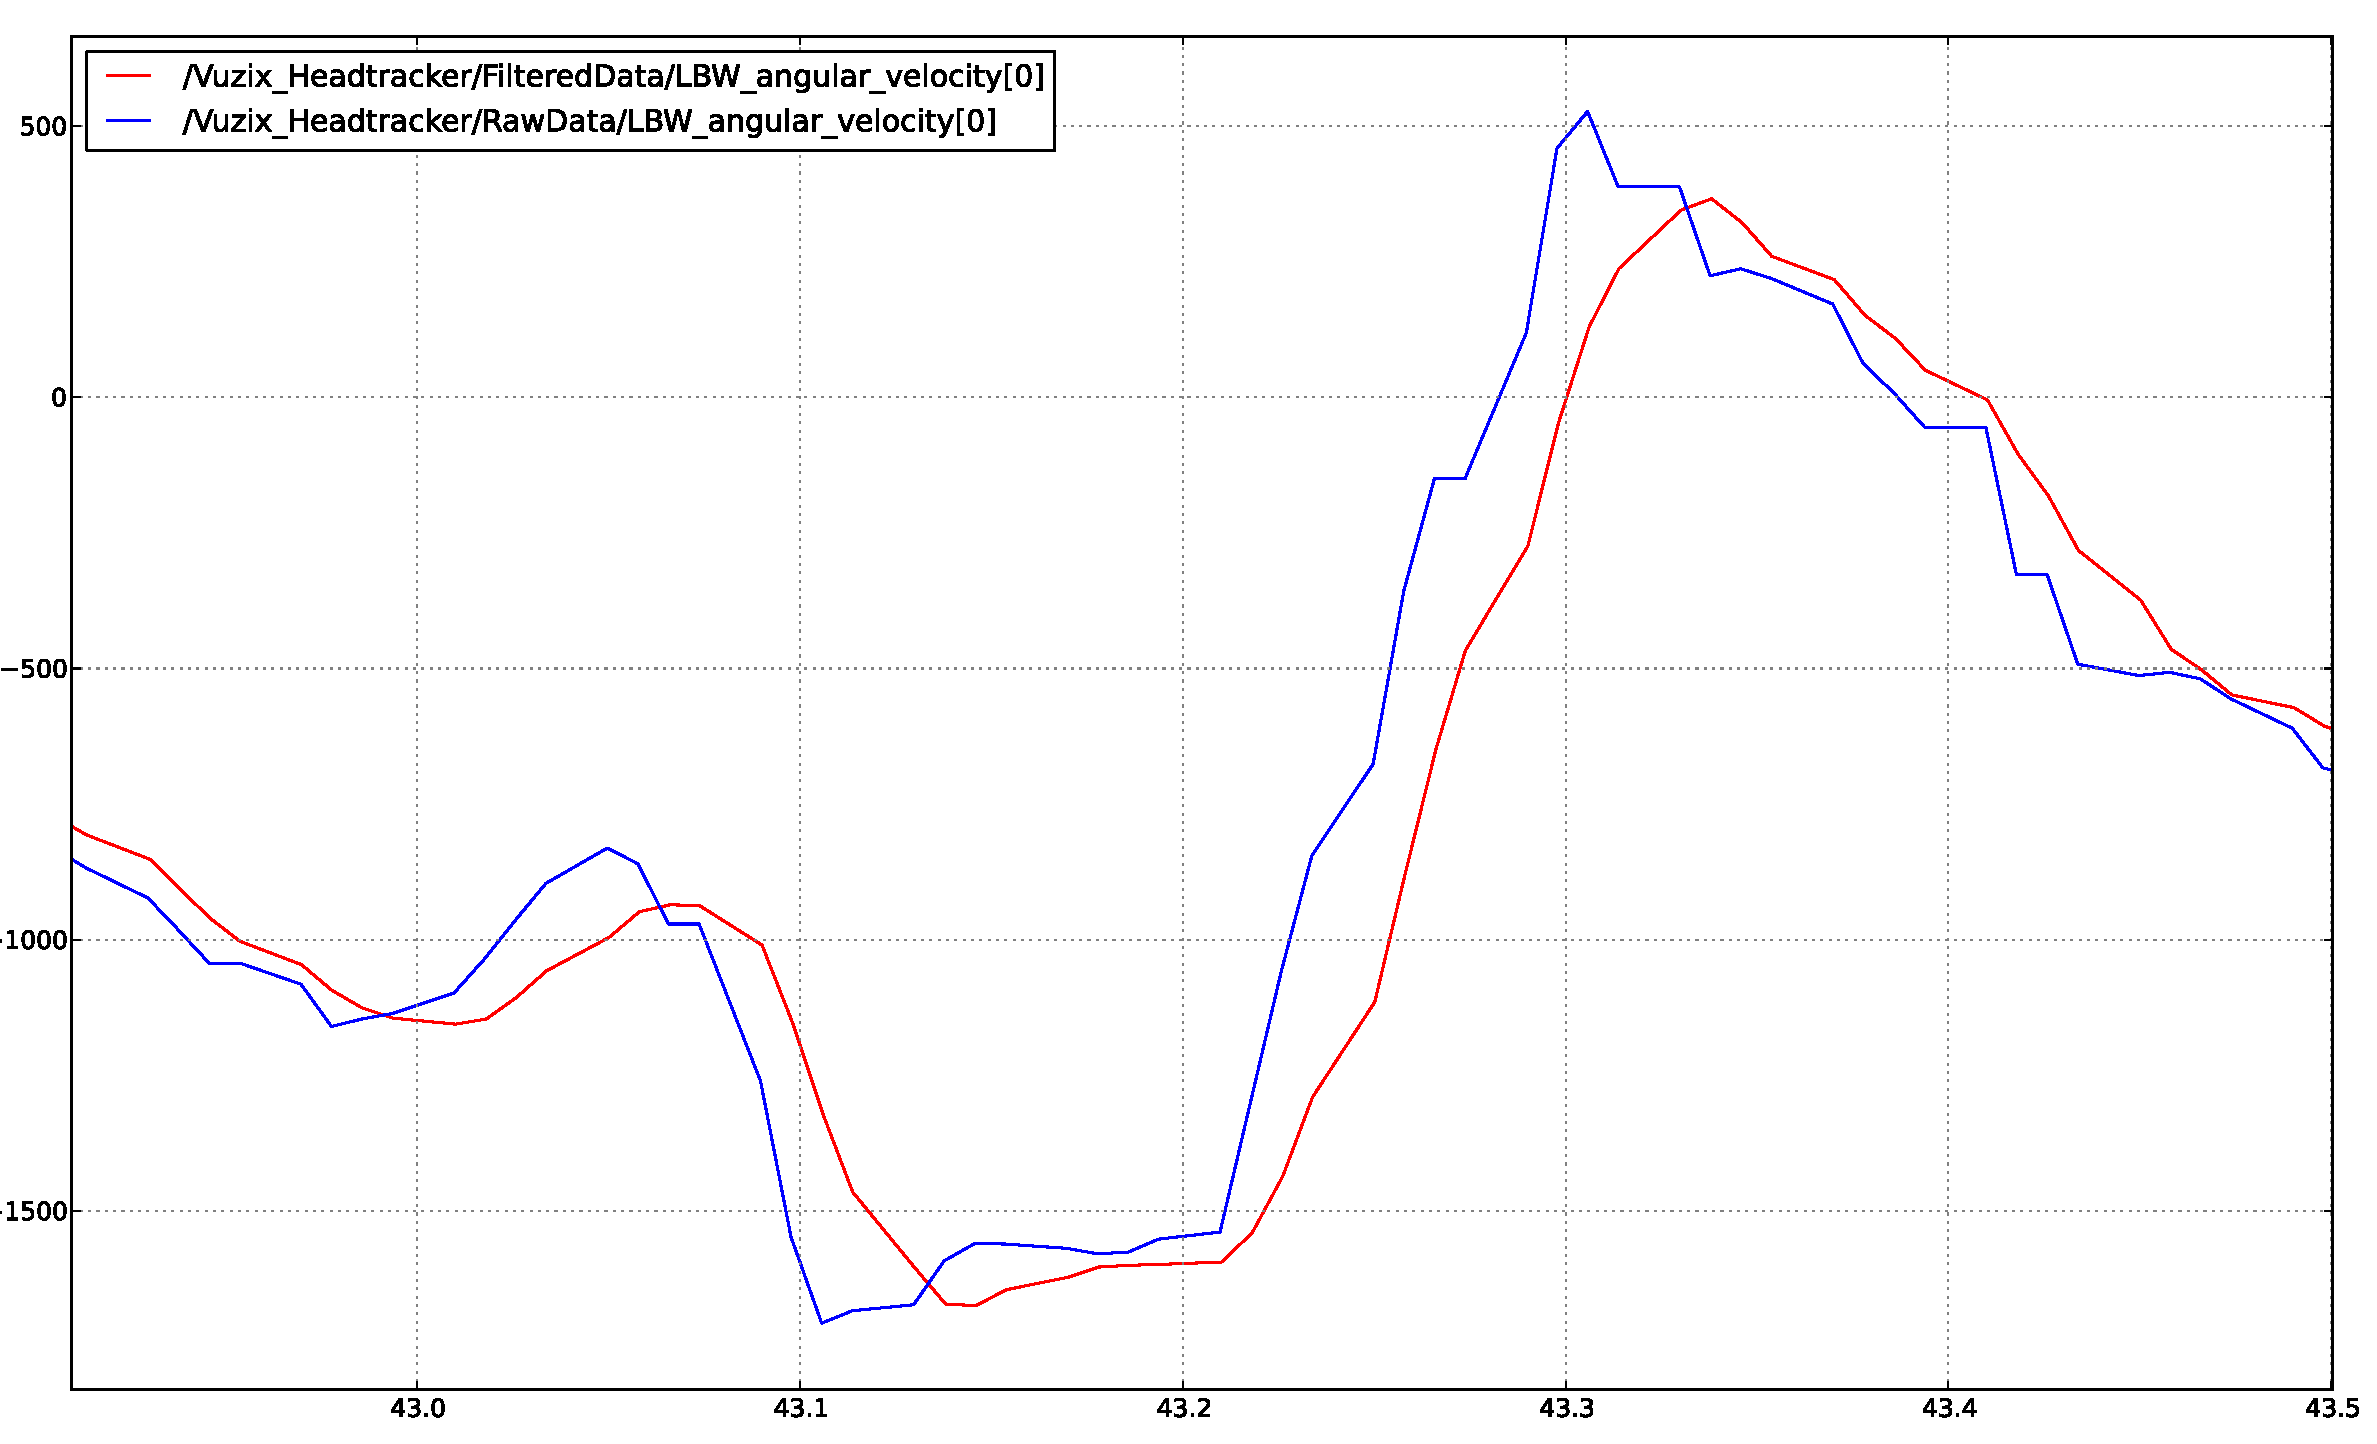
\includegraphics[width=0.45\textwidth]{FilteringDelay}
   \caption{Auswirkung des Tiefpassfilters: Ungefilterte Daten (blau) vs. gefilterte Daten (rot)}
   \label{fig:lowpass-delay}
\end{figure}

Die Wertebereiche der Gyroskope sind
in Tab. \ref{tab:ranges-gyros} aufgeführt. Beide Gyroskope liefern
einen 12-Bit-Datenwert. Somit stellt ein Zählwert des \ac{LBW}-Gyroskops eine
kleinere Veränderung dar als beim \ac{HBW}-Gyroskop.
Dies bedeutet, dass das \ac{LBW}-Gyroskop eine höhere Genauigkeit besitzt.

\begin{table}[ht]
  \centering
  \begin{tabular}{ | c | c | c | }
    \hline
    & Min. & Max. \\ \hline
    \ac{LBW} & -420   & 420   \\ \hline
    \ac{HBW} & -1680   & 1680   \\
    \hline
  \end{tabular}
  \caption{Gyroskop-Wertebereiche in $[{\degree \over s}]$}
  \label{tab:ranges-gyros}
\end{table}


Zur Fusionierung des \ac{HBW}- und \ac{LBW}-Gyroskops kommt ein einfaches Schwellwertverfahren zum Einsatz. 
Im Wertebereich, welcher von beiden Gyroskopen abgedeckt wird, werden
die Sensordaten gemittelt. Wird der Wertebereich des \ac{LBW}-Gyroskops
überschritten, wird lediglich der Wert des \ac{HBW}-Gyroskops
zurückgeliefert.

\begin{equation}
    G = \left\{
    \begin{array}{ll}
        \frac{G_{HBW} + G_{LBW}}{2}, & G_{LBW} < G_{LBW_{max}}  \\
        G_{HBW}, & G_{LBW} = G_{LBW_{max}}
    \end{array}\right. \\
\end{equation}

\todo{Die Unterscheidung deckt nicht alle Fälle ab. Was ist mit dem größer-Fall?}

Aus den gefilterten Sensordaten wird daraufhin durch Integration über
die Zeit die Orientierung berechnet. Hierzu wird die Orientierung in einem Quaternion gespeichert, welches nach jeder Sensorabtastung aktualisiert wird. Hierbei ist $dt$ die Abtastrate der Gyroskop-Sensoren, welche 100Hz beträgt.

\begin{equation}
    \Delta q = quaternion({\omega_x \over dt}, {\omega_y \over dt}, {\omega_z \over dt}) \\
\end{equation}

\begin{equation}
    q = q * \Delta q
\end{equation}

Die durch das Gyroskop berechnete Orientierung reagiert schnell auf
Änderungen. Durch die Integration entsteht in jedem Integrationsschritt jedoch ein Fehler, welcher sich summiert. Dieser Fehler wird als \emph{Drift} bezeichnet. In den folgenden Abschnitten wird beschrieben wie Beschleunigungssensor und Magnetometer verwendet werden können, um diesen Fehler zu kompensieren.

% TR: Schöner Abschnitt  :-)


\subsubsection{Beschleunigungssensor}


Der Beschleunigungssensor misst die Beschleunigung entlang der X-, Y-
und Z-Achse, im Folgenden als $acc_x$, $acc_y$ und $acc_z$ bezeichnet.
Bei stationärer Brille wird lediglich die Erdbeschleunigung $\vec g$
gemessen, somit kann aus dem Beschleunigungsvektor die Orientierung der
Brille bezüglich der horizontalen Ebene bestimmt werden. Zu beachten
ist hierbei, dass durch eine Bewegung der Brille eine zusätzliche
Beschleunigung gemessen wird, welche die berechnete Orientierung
verfälscht. Dieser Fehler ist jedoch vernachlässigbar, da die berechnete
Orientierung lediglich zur Langzeitkorrektur verwendet wird.


Zur Verwendung des Beschleunigungssensors wird zunächst wie auch beim
Gyroskop ein Tiefpassfilter angewendet, um das Rauschen der Rohdaten zu
reduzieren.
Dabei wird ein Mittelwertfilter eingesetzt.
Als Fenstergröße wird die gleiche wie beim Gyroskop gewählt, da ein ungleicher Wert zu Fehlern bei der späteren Fusion
führen würde. 

% XXX: die umrechung auf m/s2 hab ich mal rausgelassen, die ist ja glaub ich auch garnicht so wichtig und verwirrt den leser nur

Die Orientierung in Roll und Pitch kann direkt aus den Winkeln des Gravitationsvektors berechnet werden.

\begin{equation}
    roll = atan2(acc_y, acc_z)
\end{equation}

\begin{equation}
    pitch = -atan2(acc_x, \sqrt{ {acc_y}^2 + {acc_z}^2 })
\end{equation}

Die so bestimmten Roll- und Pitch-Werte sind frei von Drift, und können als Stützwerte für die aus den Gyroskopdaten berechneten Orientierungswerte verwendet werden.
Jedoch ist zu beachten, dass der Beschleunigungssensor nicht zuverlässig zur Berechnung des Yaw-Winkels verwendet werden kann.
Dies liegt darin begründet, dass sich die Sensordaten des Beschleunigungssensors nicht ändern, wenn sich der Sensor parallel zur Erdoberfläche befindet und um den Yaw-Winkel gedreht wird.


%  roll = atan2(acc_data[1], acc_data[2]);
%  pitch = -atan2(acc_data[0], sqrt(acc_data[1]*acc_data[1] + acc_data[2]*acc_data[2]));



\subsubsection{Magnetometer}
\label{headtracking_magnetometer_subsubsec}

Das Magnetometer wird im Rahmen des Praktikums zur Stützung des Yaw-Winkels (Drehung um die Z-Achse des Brillenkoordinatensystems $TF_{glasses}$) genutzt.\
Das verbaute Magnetometer misst in drei Achsen nach dem Funktionsprinzip der Wheatstoneschen Messbrücke \cite{renaudin2010complete} das Erdmagnetfeld.
Dieses Messverfahren führt zum einen zu einer kleinen und kostengünstigen Bauweise.
Zum anderen entstehen aber Messungenauigkeiten, die im Rahmen der Sensorkalibrierung beachtet und ausgeglichen werden müssen.

\begin{figure}[h]
   \centering
   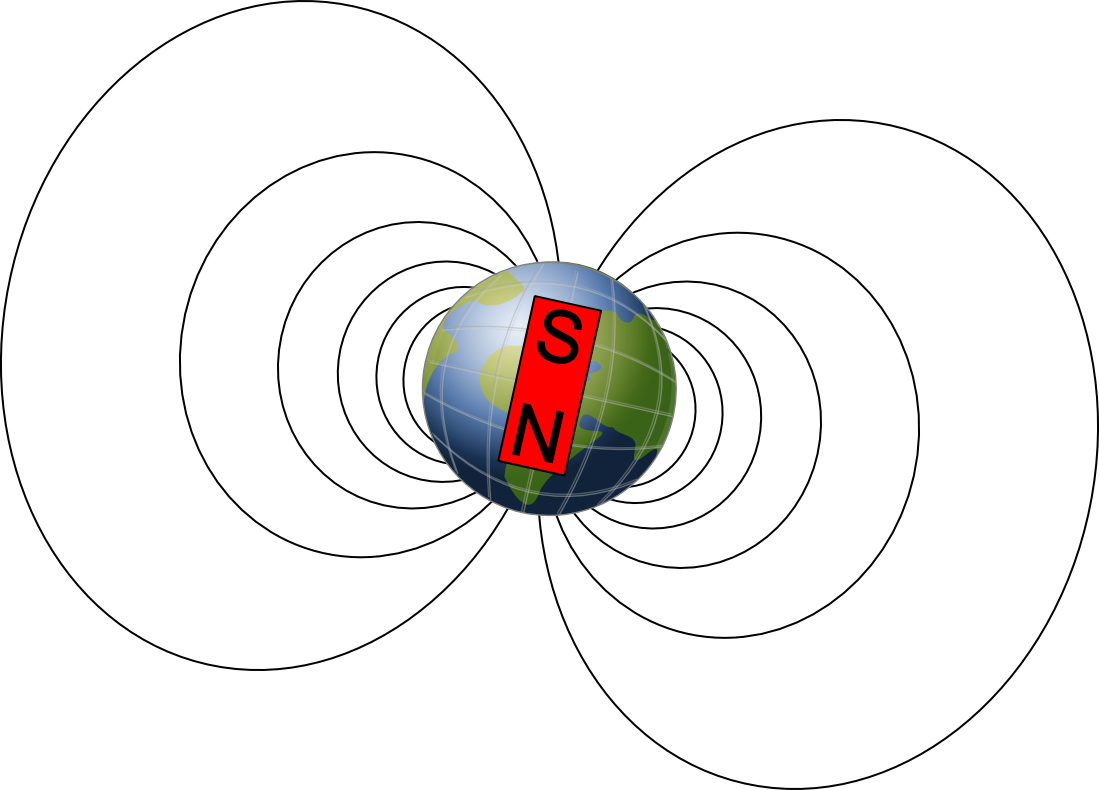
\includegraphics[width=0.4\textwidth]{earth-magnetic-field}
   \caption[mag_world]{Schematische Darstellung des Erdmagnetfelds \cite{mag_world_source}.}
   \label{fig:mag_world}
\end{figure}

\begin{figure}[h]
   \centering
   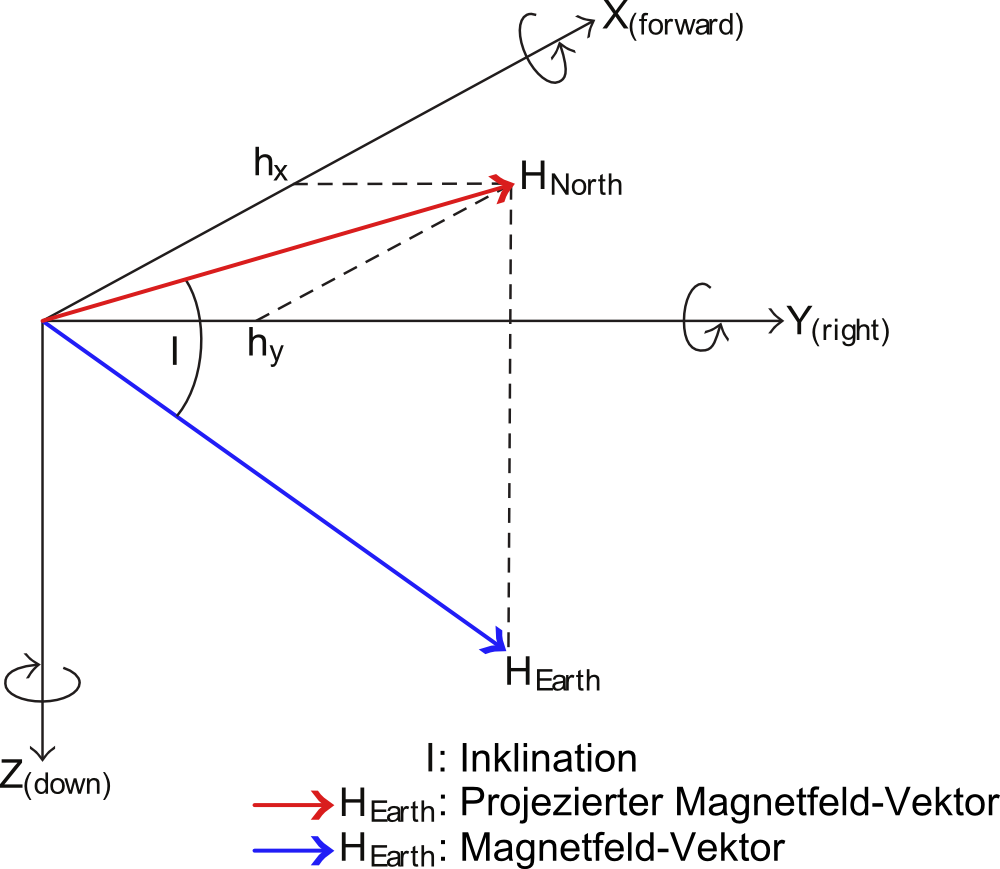
\includegraphics[width=0.4\textwidth]{magnetometer-yaw-calculation}
   \caption[mag_mapping]{Berechungsgrundlage des Magnetfeldvektors}
   \label{fig:mag_mapping}
\end{figure}
%\todo[inline]{cite Inklinationswinkel?}
%DHA: Beschreibung siehe Footnote unten

Gemessen werden die Magnetfeldlinien der Erde, welche in Abb. \ref{fig:mag_world} dargestellt sind.
Diese sind abhängig von der aktuellen Position auf der Erdoberfläche\footnote{Tatsächlich verändert sich das Erdmagnetfeld auch über die Zeit hinweg.
Diese Änderung kann aber im Rahmen des Praktikums vernachlässigt werden, da es sich um eine sehr kleine Änderung handelt (\zB für den Praktikumsort Karlsruhe ca. $1^\circ 46$'~$7.8$ arcmin/Jahr im Deklinationswinkel).}.
Sobald das Erdmagnetfeld nicht am Äquator gemessen wird, sondern im Falle des Praktikums bei etwa $49^\circ$ geographischer Breite, muss der Inklinationswinkel\footnote{Bezeichnet den Neigungswinkel des örtlichen Erdmagnetfeldes zur Horizontalen.} bei der Messung mit beachtet werden.
Dieser wird in Abb. \ref{fig:mag_mapping} mit I beschrieben.
Die Abbildung auf die XY-Ebene wird durch folgende Formel bewerkstelligt:

\begin{equation}
    \varphi = atan2(h_y,h_x)
\end{equation}

Dabei sind $h_x$ und $h_y$ die Anteile des Magnetfeldvektors $H_{Earth}$ in X- sowie Y-Richtung.

Der gemessene 3D-Magnetfeldvektor ist zunächst unkalibriert und einheitenlos.
Daher ist zuerst eine Kalibrierung der gemessenen Werte notwendig, um sie weiterverarbeiten zu können.
Diese Kalibrierung hat zum Ziel, einen kanalspezifischen Bias auszugleichen. 
Dieser entsteht durch die bereits angesprochenen Messungenauigkeiten des Sensors sowie durch sogenannte \textit{Hard Iron} Störeffekte, welche durch eigenständige Magnetquellen induziert werden.
Beispiele für diese Störeffekte sowie die letztlich kalibrierten Daten sind in Abb. \ref{fig:mag_kugel_plots} als Kugelplots dargestellt.

\begin{figure}[ht]
\centering
\subfigure[Unkalibrierte Magnetometerdaten mit Hard Iron Störeinflüssen]{
    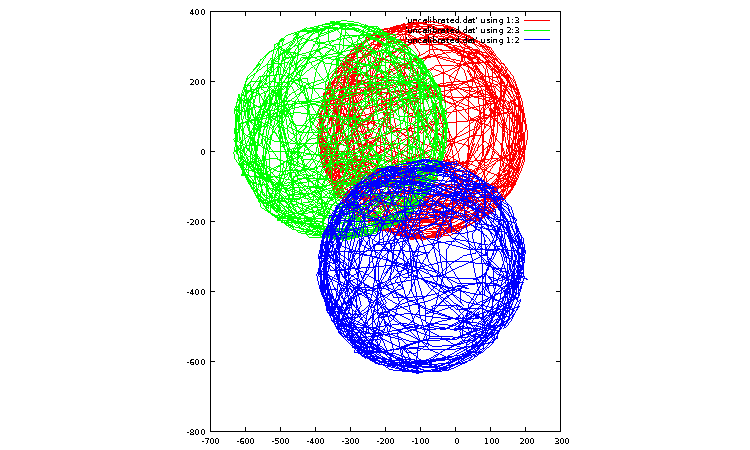
\includegraphics[width=0.5\textwidth]{uncalibrated}
    \label{fig:subfig1}
}
\subfigure[Kalibrierte Magnetometerdaten]{
    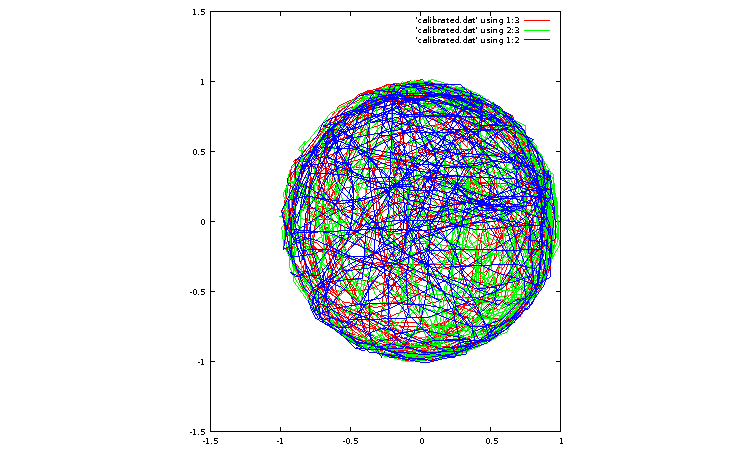
\includegraphics[width=0.5\textwidth]{calibrated}
    \label{fig:subfig2}
}

\caption[]{2D-Sichten auf Kugel aus Magnetometerdaten}
\label{fig:mag_kugel_plots}
\end{figure}

Im Gegensatz zu den bisher vorgestellten Sensoren wird die Kalibrierung des Magnetometers durch Bewegung durchgeführt.
Ziel ist es, die Wertebereiche in allen drei Achsen zu erfassen.
Dafür wird die Brille in allen Achsen um mindestens $360^\circ$ gedreht, um die minimalen und maximalen Werte zu registrieren. 
Des Weiteren werden die Daten noch durch einen Tiefpassfilter geglättet, sowie auf einen Wertebereich von $[-1,1]$ abgebildet.
Der Tiefpassfilter wird wie in Abs. \ref{headtracking_imu_gyro_subsubsec} bereits beschrieben durchgeführt. 
Die Anwendung der Kalibrierung und Normierung wird durch nachfolgende Formel bewerkstelligt:
\begin{equation}
    m_{norm} = \frac{m_{raw}- \frac{m_{\delta}}{2}}{2~m_{\delta}}, {\scriptstyle mit~m_{\delta}~=~m_{max}~-~m_{min}}
\end{equation}
Dabei bezeichnet $m_{norm}$ einen normierten Magnetfeldvektorkanal, $m_{raw}$ die Rohdaten des jeweiligen Kanals und $m_{\lbrace max, min\rbrace}$ den gemessenen Maximal- bzw. Minimalwert.

Ursprünglich war die Verwendung des Magnetometers zur Stützung des Yaw-Winkels fraglich, da der Einsatz im Versuchsträger \emph{CoCar} viele magnetische Störquellen in Form der vorhandenen Boardtechnik vermuten lies. 
Allerdings konnten durch mehrere Testläufe im Fahrzeug keine größeren Störeffekte gemessen werden. Trotz allem muss eine Kalibrierung in einem möglichst störfreien Umfeld durchgeführt werden, da durch Störquellen (wie bspw. ein Dauermagnet, eine Tastatur, \oae) die Messdaten wie in Abb. \ref{fig:uncalibrated_error} zu erkennen wesentlich beeinflusst werden. In Abb.~\ref{fig:uncalibrated_error} sind unkalibriete Messdaten dargestellt (Kreise liegen nicht über einander). Die Störungen sind dadurch zu erkennen, dass sie außerhalb der Kreise der einzelnen Kanäle liegen.

\begin{figure}[ht]
	\centering
    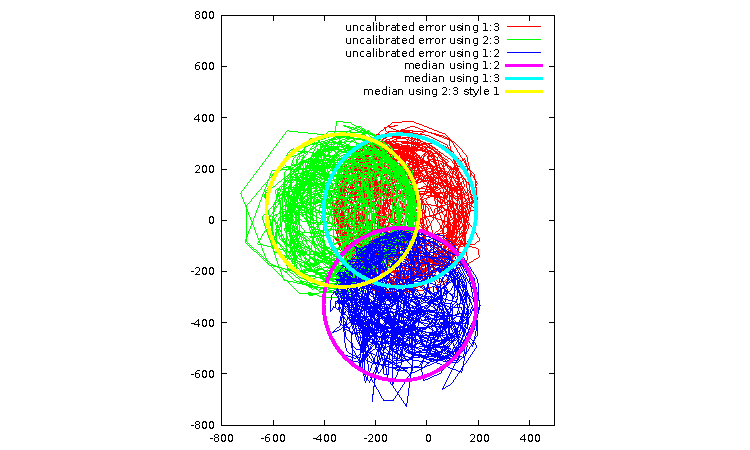
\includegraphics[width=0.5\textwidth]{uncalibrated_error}
	\caption[]{2D-Sichten auf Kugel aus Magnetometerdaten mit Störquelle}
	\label{fig:uncalibrated_error}
\end{figure}

Um die Magnetometerdaten letztlich zur Stützung des Yaw-Winkels zu nutzen, werden die Daten zuerst in das Weltkoordinatensystem transformiert.
\todo{Es geht nicht hervor welche Daten hier gemeint sind: Nur Mag oder auch Gyro, Acc? Hat das auch wieder mit der 15-Grad-Verdrehung zu tun? Haben die Implementierung leider grad nicht hier zum Nachschauen ;)}
Danach wird das vorhandene Rotationsquaternion $q_{gyro,acc}$ mit $q_{mag}$ (Magnetometer-Quaternion) interpoliert.
Das genaue Verfahren wird im nachfolgenden Abs.~\ref{headtracking_fusion_subsec} vorgestellt.
